\chapter{Parameterization of Human Knee Joints}
\label{sec:KneeParams}

The proposed and prototyped knee joint requires a specific input of patient parameters to achieve its goal of matching a person's knee movement. Therefore, a system must be developed to non-invasively identify a relationship between the flexion of the patient's knee joint and the linear movement of the shank away from the knee's joint center. There have been several attempts to parameterize the human knee joint using many different methods, including \cite{3DKinKneeJointOldStabby}, \cite{MRIKneeShape_Unloaded}, \cite{MRIKneeShape_Loaded}, and \cite{ModelAnalysisDeepKneeFlexion}. All of these studies focus on the tibiofemoral relationship, i.e. the bone movement within the lower limbs. However, rehabilitation exoskeletons connect to the skin of its user. Other studies have identified a difference between identifying knee kinematics through skin markers and bone pins \cite{reinschmidt1997effect}, suggesting there is in fact a distinct difference between tibiofemoral movement and skin movement around the knee. Therefore, an imaging workflow and software processing program needs to be developed to be able to parameterize a patient's knee movement with consideration to skin movement.

To identify the knee relationship, an imaging workflow as well as an accompanying software analysis tool is proposed and tested with pilot data. This imaging method uses a motion capture system to identify movement of specific markers attached to a person's skin. This will all be processed using a custom software workflow consisting of both Vicon image processing and custom Python scripts that will extract the parameters from the data. To test this workflow, an experiment is proposed using medical MR imaging to identify the kinematics of the knee joint, compare the developed knee joint to a traditional pin joint, and determine the relationship between the knee joint kinematics and the skin movement surrounding the knee.

\section{Proposed Method of Imaging}
\label{sec:ImaginKneeProcedure}

\begin{figure}[ht!]
    \centering
    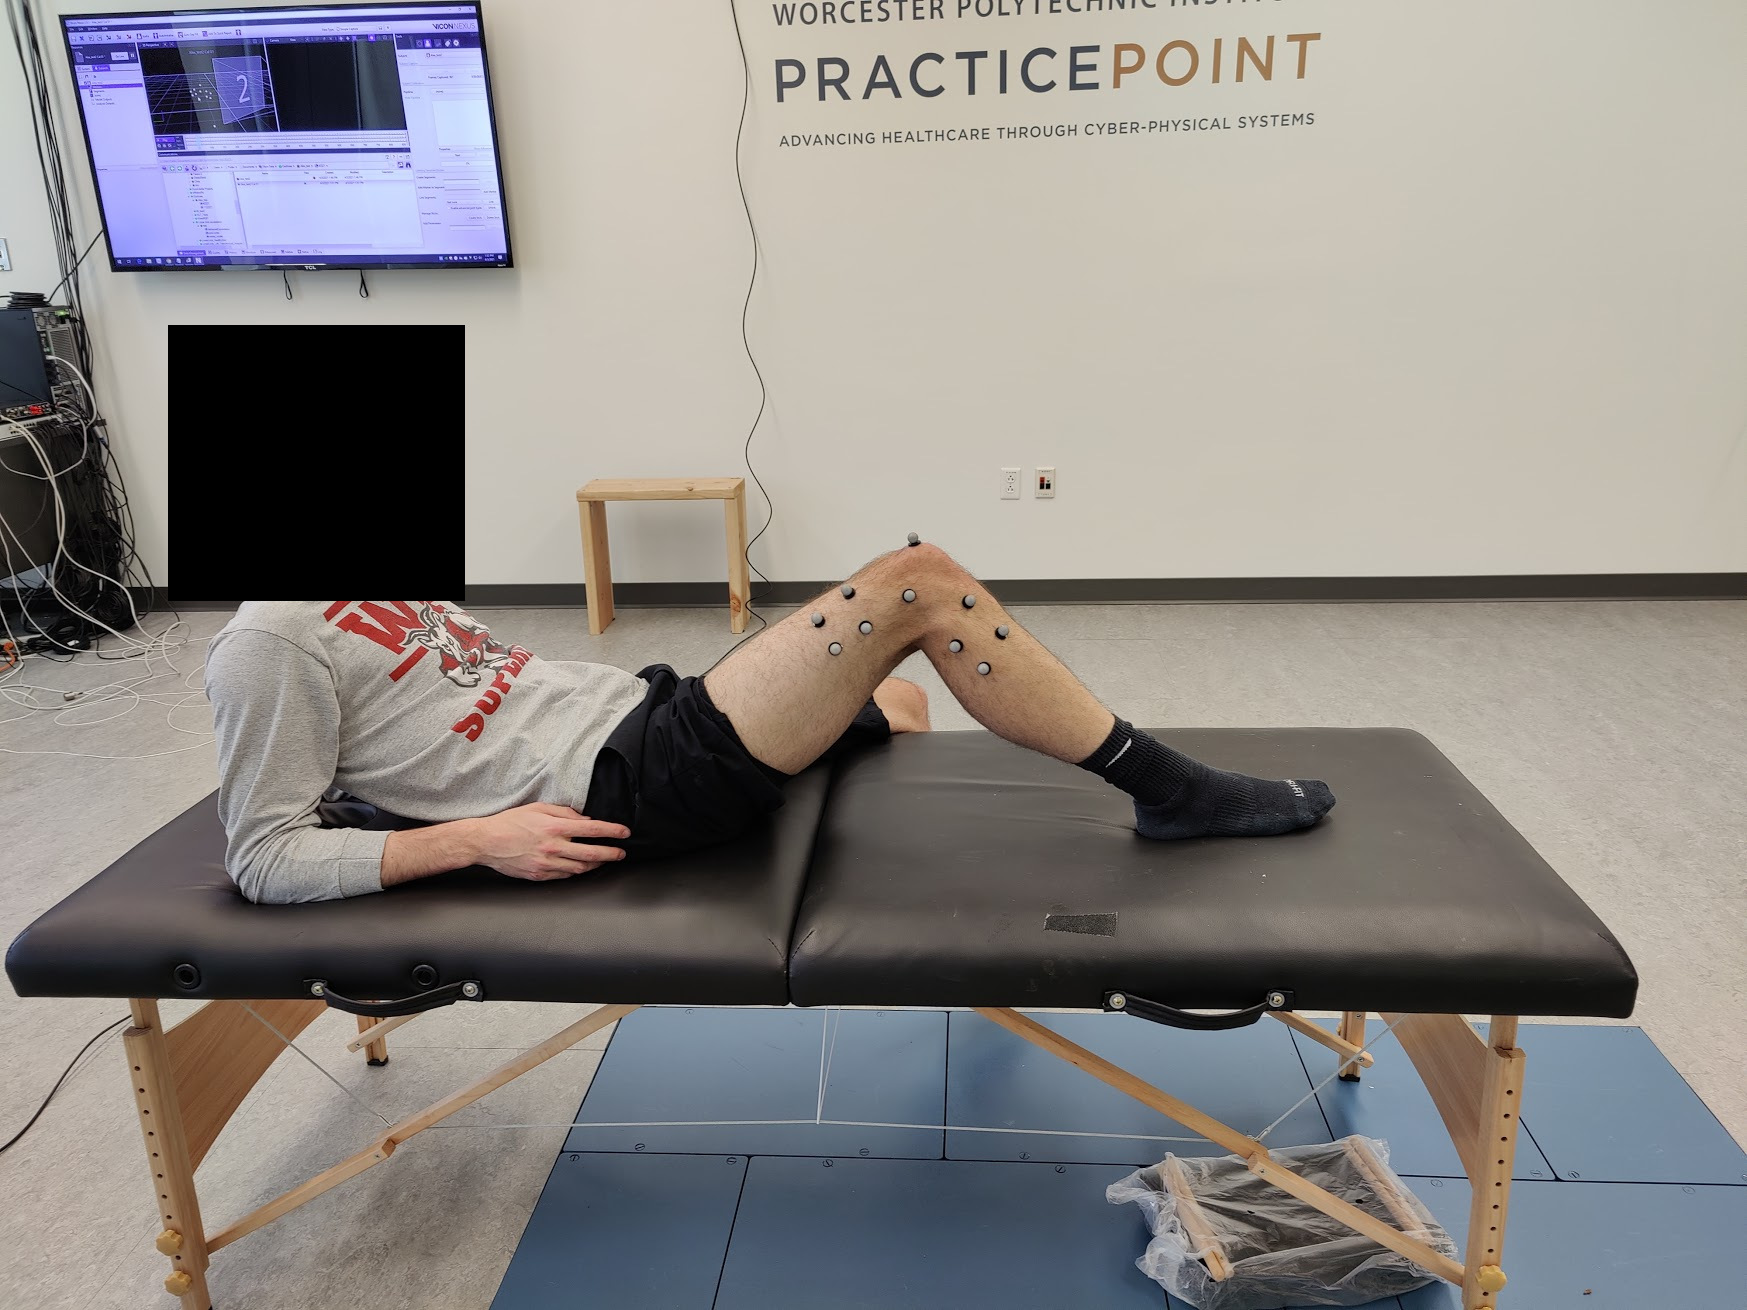
\includegraphics[width=0.65\textwidth]{Figures/Param/StudyPatientPositioning.jpg}
    \caption{Depicts the patient position during motion capture. The patient will then flex and extend their knee while keeping the heel on the table.}
    \label{fig:ParamPatientPosition}
\end{figure}

The proposed imaging workflow can be split up into two major parts: the imaging session and the software processing. For flexibility and speed, the usage of a motion capture system is proposed, which can develop accurately track the position of motion dots. In this study, the motion capture system used was a 10-camera Vicon Vantage 5 \footnote{See Vicon system here: \url{https://www.vicon.com/hardware/cameras/vantage/}}, but any motion capture system is usable given enough precision. 

To measure the knee flexion, a patient is placed on their back, shown in \autoref{fig:ParamPatientPosition}.Motion capture dots are then placed on the patient using double-sided tape to track the positions where the exoskeleton will attach to the skin. Two additional points can be placed on the knee for extra feedback and the final joint position, but are not necessary for the software system. Then, the patient will flex and extend their knee joint while keeping the heel on the table to stabilize the knee and prevent shanking. The placement of the patient should allow for a technician to help the patient bend their knee if their condition does not allow them to do so themselves. Once the data is collected, it can be processed by the parameterization software system.

\section{Parameterization Software}
% TODO: Add software flowchart
The collected data first goes through a Vicon workflow for processing. This will properly format the data, create virtual joints, and determine joint centers. This is done using the built-in tools called SCoRE (Symmetrical Center of Rotation Estimation) and SARA (Symmetrical Axis of Rotation Analysis). Additionally, a built-in tool will determine the angle of the knee joint using the four dots on each section of the patient's leg. This Vicon specific workflow can be exported, shared, and reused for others who are using a similar system. The output of the workflow is a CSV file which can be parsed by a custom script.

To finish the parameterization of the knee, custom software was developed and written in Python. This software utilizes the AiM Vicon Python module \footnote{The AiM Vicon Python module is an open-source project found here: \url{https://github.com/WPI-AIM/AIM_Vicon}} which parses the CSV file from above. The joint angle, SARA, SCoRE, and marker positions are extracted from the data and placed in their specified datatypes. Since the AiM Vicon module did not have all the tools needed for this project, I developed and contributed to the Python module. Additional features added include SARA and SCoRE support, a new 3D visualizer, and stability improvements when importing different workflows.

\begin{figure}[ht!]
    \centering
    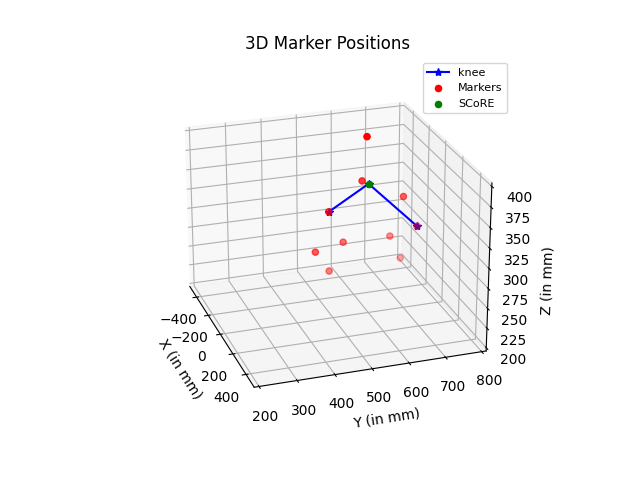
\includegraphics[width=\textwidth]{Figures/Param/3D_Marker_Animation.png}
    \caption{An example of a possible output from the Parameterization Software System shown in a visualizer}
    \label{fig:SoftwareSampleData}
\end{figure}

With the data parsed and imported, the final step is to calculate the final joint angles and determine the linear extension between the thigh and shank. The axis of rotation from SCoRE and all marker positions are projected onto a plane, which is calculated to be approximately the same as the plane of the manufactured joint. Then the final distance and angle are calculated by drawing two virtual lines as shown in \autoref{fig:SoftwareSampleData}: 1. from the projected primary thigh marker to the projected SCoRE location and 2. from the projected SCoRE location to the projected primary shank marker. The lengths of these lines then become the calculated linear extension and the angle between these two lines become the flexion. These two metrics are then combined into a dataset, and a best fit quartic curve is selected to become the patient's knee parameters.

\section{Testing with Pilot Data}
Due to time constraints, IRB (Internal Review Board) approval was not obtained to run a full study. However, some data was used to develop the software platform that will analyze the data. The graphs in \autoref{fig:Subj1KneeParams} and \autoref{fig:Subj2KneeParams} show the relationships between the knee joint flexion (angle of the knee) and the linear extension (distance of the shank to the joint center).

\begin{figure}[ht!]
    \centering
    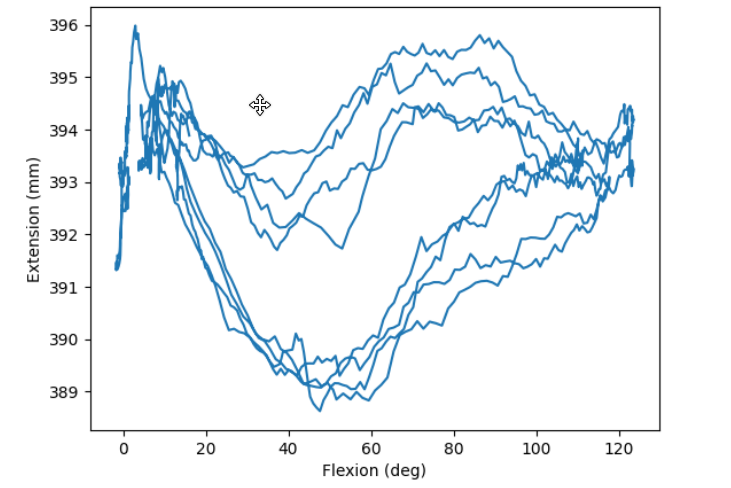
\includegraphics[width=\textwidth]{Figures/Param/Subj1_KneeProfile.png}
    \caption{A visualization of the angular flexion and linear extension of the shank from the joint center of the first dataset with subject 1. Subject bent and extended their knee joint 4 times.}
    \label{fig:Subj1KneeParams}
\end{figure}

\begin{figure}[ht!]
    \centering
    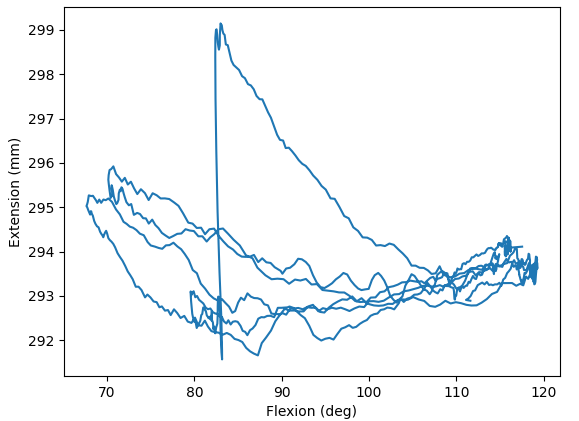
\includegraphics[width=\textwidth]{Figures/Param/Subj2_KneeProfile.png}
    \caption{A visualization of the angular flexion and linear extension of the shank from the joint center of the second dataset with subject 2. Subject bent and extended their knee joint 3 times.}
    \label{fig:Subj2KneeParams}
\end{figure}

The data displayed in \autoref{fig:Subj1KneeParams} has a variation of up to \(7mm\) for any given angle. However, what is most interesting is the difference in the direction of the flexion. When the knee joint angle is increasing (knee is being bent), the markers are closer together, compared to when the knee joint is decreasing. In any given direction of movement, variation is less than \(2mm\), suggesting that this seemingly cyclical trajectory is not due to measurement variations or inaccuracies.

\autoref{fig:Subj2KneeParams}'s data is seemingly less dependent on the knee joint angular velocity direction. All data is within a \(3mm\) variation at any given angle. The notable exception is the \(7mm\) spike that can be seen at roughly \(25^\circ\) mark. This can likely be explained by either an accidental shift in the markers or a slight measurement error in the motion capture system. However, there is not sufficient data to make a conclusion as to the reasoning.

The data analyzed both show that the maximum variation in skin movement through the flexion of the knee never exceeded \(7mm\), even with the outlier event from \autoref{fig:Subj2KneeParams}. In comparison, studies presented in \autoref{sec:KneeModel} describe a tibio\-femoral relationship that varies over \(40mm\) throughout the joint flexion. While these two data points are not statistically significant enough to make a conclusion for all human knees, the preliminary pilot data suggests that the skin movement is different than the tibiofemoral movement. An in-depth study is needed to make a definitive conclusion.

\section{Study Outline}

As a part of this thesis, an study was designed to test the developed parameterization software as well as the knee joint's capability to be customized to a specific person. However, due to time constraints, IRB (Internal Review Board) approval to run the human study was not obtained, and therefore the study was not run. The study's methodology is outlined below, and the IRB proposal documents are attached in \autoref{apx:ParamStudyDocs}.

Up to 6 subjects are to be selected to partake in this study. Each subject should not have any prior severe knee injury, and should be cleared to be imaged with an MRI. The study will start with imaging the knee using the motion capture procedures outlined in \autoref{sec:ImaginKneeProcedure}, and parameters will be selected using the parameterization software developed. These parameters will be used to manufacture an MRI safe personalized knee joint. Additionally, a second non-personalized pin joint will be manufactured and used as a control.

The second stage of the study will compare the fit of the two joints. The subject will undergo MR scans at up to 3 different knee angles, first with no joint and then subsequently with each type of joint. The movement (if any) of the joint in reference to the subjects body will be measured. A successful experiment should demonstrate that the customized knee joint moves less than a non-customized pin joint. Additionally, the tibiofemoral movement can be compared to the measured parameters to determine how much the skin moves relative to the knee joint.
